\documentclass{beamer} %[12pt]
\usepackage{xcolor}
%\usetheme{boadilla}
%\usetheme{malmoe}
%\usetheme{copenhagen}
%\usecolortheme{rose}
\usecolortheme{beaver}
\usepackage{pgf, graphics}
\usepackage{graphicx}
%\usepackage[left=3cm,top=3cm,right=3cm,nohead,nofoot]{geometry}
\usepackage{hyperref}
\usepackage{setspace}
\usepackage[square]{natbib}
\usepackage{amsmath}
\usepackage{amssymb}
\usepackage{verbatim}
\usepackage{color}
\usepackage{fancyvrb}
\usepackage{bbm}

\begin{filecontents}{ref.bib}
\end{filecontents}

%\usetheme{EastLansing}
%\usepackage{natbib}
\bibliographystyle{apalike}
% make bibliography entries smaller
%\renewcommand\bibfont{\scriptsize}
% If you have more than one page of references, you want to tell beamer
% to put the continuation section label from the second slide onwards
\setbeamertemplate{frametitle continuation}[from second]
% Now get rid of all the colours
\setbeamercolor*{bibliography entry title}{fg=black}
\setbeamercolor*{bibliography entry author}{fg=black}
\setbeamercolor*{bibliography entry location}{fg=black}
\setbeamercolor*{bibliography entry note}{fg=black}
% and kill the abominable icon
\setbeamertemplate{bibliography item}{}


\newcommand{\hl}[1]{\colorbox{yellow}{#1}}
\newcommand{\hlblue}[1]{\colorbox{green}{#1}}
\newcommand{\hlblu}[1]{\colorbox{cyan}{#1}}
\newcommand{\hlred}[1]{\colorbox{cyan}{#1}}
\newcommand{\hlre}[1]{\colorbox{pink}{#1}}
\newcommand{\hlgreen}[1]{\colorbox{pink}{#1}}
\newcommand{\hlgree}[1]{\colorbox{green}{#1}}



\DeclareMathOperator*{\argmax}{\arg\!\max}

\DeclareMathOperator*{\argmin}{\arg\!\min}


\newcommand{\specialcell}[2][c]{%
  \begin{tabular}[#1]{@{}c@{}}#2\end{tabular}}



%\setbeamersize{text margin left=.5cm,text margin right=.5cm}
\newenvironment{changemargin}[2]{%
  \begin{list}{}{%
    \setlength{\topsep}{0pt}%
    \setlength{\leftmargin}{#1}%
    \setlength{\rightmargin}{#2}%
    \setlength{\listparindent}{\parindent}%
    \setlength{\itemindent}{\parindent}%
    \setlength{\parsep}{\parskip}%
  }%
  \item[]}{\end{list}}
\setbeamertemplate{navigation symbols}{}%remove navigation symbols
\usepackage{color}
\newcommand{\hilight}[1]{\colorbox{yellow}{#1}}
\setbeamertemplate{footline}[page number]

\begin{document}


\title[dedup]{Today:  High-D Continuous Data, Clustering}


\author[Samuel L. Ventura]{\\
  \large{Sam Ventura\\36-315\\Today:  Distance Matrices, \\Hierarchical Clustering, Dendrograms}}
\institute[CMU Statistics]{Department of Statistics\\Carnegie Mellon University}
\date{October 24, 2016}


\begin{frame}
	\maketitle

	
\end{frame}



\begin{frame}\frametitle{Distance = Metric = Distance Metric = Distance Function}
	\small
	
	Function that defines distance between pairs of observations in a dataset
	
	\vskip 0.35 cm
	
	\textbf{Properties}:
	
	\vskip 6 cm
	
	Examples:  
	
\end{frame}


\begin{frame}\frametitle{Distance Matrices}
	\small
	
	A \textbf{distance matrix} is a data structure that efficiently organizes the pairwise distances between all observations in a dataset.
	
	\vskip 0.5 cm
	
	Pairwise distances are organized into the lower-triangle of a matrix, $D$
	
	\vskip 0.5 cm
	
	The $(i,j)^{th}$ element of the matrix contains the distance between $x_i$ and $x_j$:
	
	\vskip 0.25 cm
	
	$D[i,j] = d(x_i, x_j)$
	
	\vskip 0.5 cm
	
	Examples:
	
	
	
	\vskip 10 cm
	
	

	
\end{frame}


\begin{frame}\frametitle{Dendrograms / Visualizing High Dimensional Structure}
	\small
	\centering
	
	There is no easy way to visualize how far apart observations are in high-dimensional space.  One option we do have:  \textbf{Dendrograms}
	
	\vskip 0.25 cm
	
	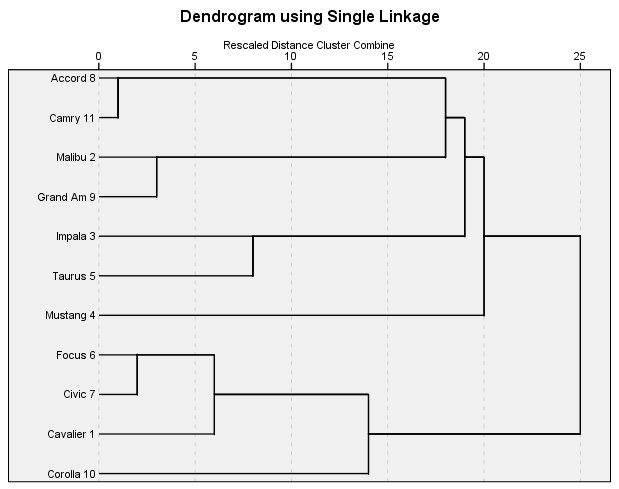
\includegraphics[width = 0.81\linewidth]{dendro.jpg}
	
\end{frame}



\end{document}
